Der er en række interessenter at tage hensyn til, når det kommer til hvordan et skema skal lægges. Nogle skal planlægge skemaet, som har krav til skemaet og dets indhold og andre skal følge det. For at lave et program der kan bruges, skal der tages højde for de forskellige interessenterne skal bruge programmet, og derfor skal det først undersøges hvordan de forskellige interessenter bliver påvirket af en softwareløsning, og hvad de gerne vil have ud af en softwareløsning. 


Kommunernes mål er at forbedre elevernes læring samt overholde undervisningsministeriets krav. Både uddannelsesministeriet og kommunen visse krav til hvilke fag der skal skrives på skemaet og hvor mange lektioner der skal afsættes til de forskellige fag. De vil ikke kunne mærke en forskel hvis der kom en software løsning.\footfullcite{lov2016}


Skolelederen arbejde ud for et budget, som han får tildelt af kommunen og derfor interesseret i at optimere forbruget. Derfor ville en softwareløsning som kunne reducere timeantallet det tager at ligge skema have stor interesse hos skolelederen. Softwareløsningen ville gøre det muligt at bruge de sparede penge andre steder på skolen hvor de ville have mere gavn. Skolelederen har stor indflydelse på om programmet nogensinde bliver til noget, da det er skolelederen som skal vælge at investere i programmet. Hvis skolelederen ikke siger god for at ligge kapital til programmet vil det ikke blive til noget. Det ville også kræve at programmet fungere fejlfrit, da skolelederen ikke har interesse i at investere i en softwareløsning som skaber flere problemer end det løser. Så skolelederen er interesseret i en softwareløsning som gør, at skemaet fungerer uden problemer, da det er skolelederen der står til ansvar hvis programmet laver fejl.\footfullcite{interview}


Lærerne bruger rigtig mange kræfter og tid på at lægge skema.\footfullcite{interview} En softwareløsning ville tage noget af arbejdsbyrden fra lærernes skuldre og sørger for at de kan fokusere fuldt ud på undervisningen. Lærerne vil have ret stor indflydelse på hvordan en softwareløsning vil komme til at se ud, da det er dem som lægger skemaet. Lærerne vil også have stor indflydelse på om en softwareløsning vil blive implementeret på en skole, da softwareløsningen skal kunne opfylde lærernes betingelse for et skoleskema fejlfrit, da lærerne ikke er interesseret i et program som skaber flere problemer for dem end det reelt løser. Lærernes betingelser til et software program består i at få et optimeret skemaet, så deres elever er fokuseret, når de skal modtage undervisning. Samt hensyn til at underviserens forberedelsestimer ligger sammenlagt i stedet for enkeltvis. Derudover har skolen fundet ud af, at eleverne ikke kan koncentrere sig i de tungere fag over middag, så de tunge fag bliver oftest placeret før middag. En softwareløsning ville også have en stor påvirkning på lærernes hverdag, da de arbejde ud fra skoleskemaet og alle problemer som skoleskemaet skaber ville have direkte påvirkning på lærerne.\footfullcite{interview}


Eleverne har ingen interesse i en softwareløsning, og vil ikke have en indflydelse på hvordan den endelige løsning kommer til at se ud, da de ikke har en fingre med i spillet når det kommer til skemaplanlægning. Eleverne vil dog blive påvirket kraftigt af en softwareløsning, da det ville ændre deres skema som de følger dagligt, og et dårligt lagt skema vil gøre at de F.eks. Ikke har energi til at komme igennem dagen, hvis der bliver lagt for mange tunge fag på en dag.


Forældrene er interesseret da det er deres børn der bliver påvirket. Det er ofte meget vigtigt for forældrene, at deres børn har det godt i skolen, og at de ikke kommer trætte hjem så de har overskud til aktiviteter udenfor skolen. Derudover ønsker forældrene også, at deres barns skema er optimeret, så barnet får mest muligt fagligt ud af at gå i skole. Forældrene har dog ingen påvirkning på hvordan skemaet bliver lagt, og derfor ikke vil opdage hvis skolen begynder at bruge en softwareløsning til at gøre arbejdet.\footfullcite{interview}
For at overskueliggøre de forskellige interessenter og deres indflydelse på, hvordan skemaet bliver bygget, og hvilken påvirkning skemaet vil have på dem, kan de forskellige interessenter opstilles i følgende skema:
\begin{figure}[!h]
  \centering
  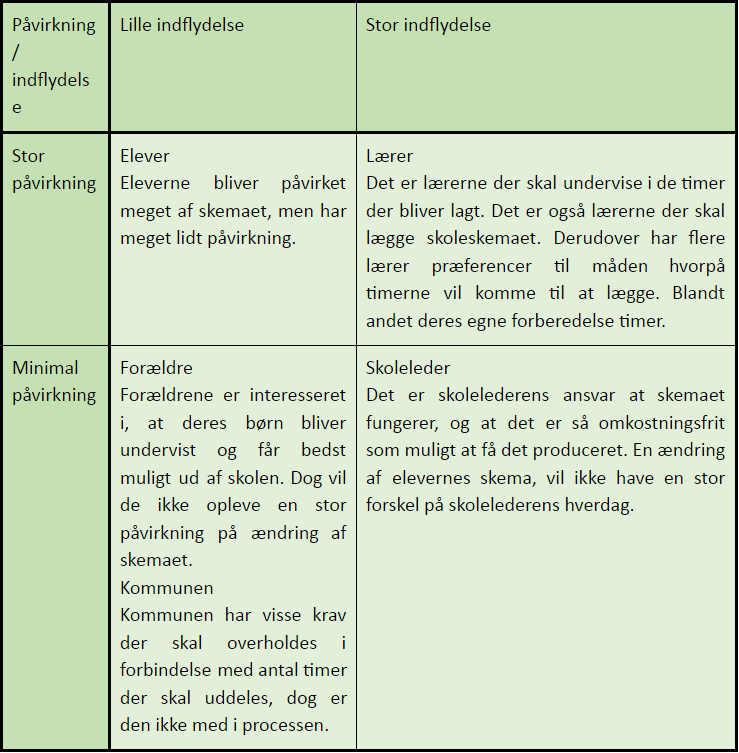
\includegraphics[width=\textwidth]{partials/graphics/interessentanalyse.png}
  \caption{Model over de indblandede interessenter.}
  \label{fig:interessenter}
\end{figure}
